\tikzset{
    vert/.style = {
        draw,
        circle,
        inner sep = 1pt,
        minimum size = 10pt
    }
}


    
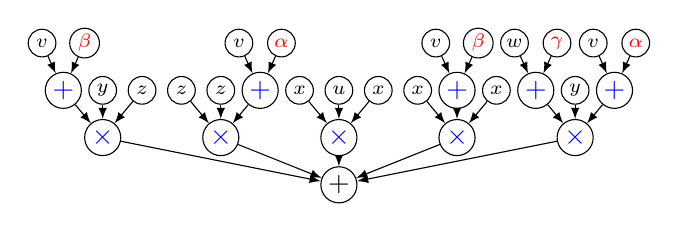
\begin{tikzpicture}[>=latex]
    \pgfmathsetseed{100011}


    \def\vars{{"$x$","$y$","$z$","$u$","$v$","$w$"}}
    \def\cons{{"$\alpha$","$\beta$","$\gamma$"}}
    
    \node[vert] (a) at (0, 0) {$+$};

    \foreach \i in {1, 2, ..., 5}{ 
        \node[vert] (b) at ({1.5 * (\i - 3)}, 0.6) {\textcolor{blue}{$\times$}};
        \foreach \j in {1, 2, 3}{
            \pgfmathsetmacro\inp{int(round(5 * abs(rand)))}
            \ifnum \inp < 4
                \node[vert] (c) at ({1.5 * (\i - 3) + 0.5 * (\j - 2)}, 1.2)
                    {\scriptsize \pgfmathparse{\vars[\inp]}\pgfmathresult};
            \else
                \node[vert] (c) at ({1.5 * (\i - 3) + 0.5 * (\j - 2)}, 1.2) {\textcolor{blue}{$+$}};
                \node[vert] (d1) at ({1.5 * (\i - 3) + 0.5 * (\j - 2) - 0.27}, 1.8)
                    {\scriptsize \pgfmathparse{\vars[\inp]}\pgfmathresult};
                \pgfmathsetmacro\inp{int(round(2 * abs(rand)))}
                \node[vert] (d2) at ({1.5 * (\i - 3) + 0.5 * (\j - 2) + 0.27}, 1.8)
                    {\scriptsize \textcolor{red}{\pgfmathparse{\cons[\inp]}\pgfmathresult}};
                \draw[->] (d1) -- (c);
                \draw[->] (d2) -- (c);
            \fi
            \draw[->] (c) -- (b);
        }
        \draw[->] (b) -- (a);
    }
\end{tikzpicture}